% 附录
% 如果不需要附录，可以删除此文件或注释掉 main.tex 中的引用

\chapter{攻读学位期间发表的学术论文}

\begin{enumerate}
    \item 张三, 李四. 基于深度学习的图像识别算法研究[J]. 计算机科学与探索, 2024, 18(5): 123-135.
    \item 张三, 王五, 李四. 一种轻量化卷积神经网络的设计与实现[C]// 第33届中国机器学习会议论文集. 2024: 456-467.
\end{enumerate}

\chapter{补充实验数据}

\section{网络各层详细参数统计}

表\ref{tab:layer_params}列出了本文提出的网络模型各层的详细参数分布情况。

\begin{table}[htbp]
    \centering
    \caption{网络各层参数统计}
    \begin{tabular}{cccc}
        \toprule
        \textbf{层类型} & \textbf{数量} & \textbf{参数量(M)} & \textbf{占比(\%)} \\
        \midrule
        $1\times1$ 卷积 & 12 & 0.82 & 25.6 \\
        $3\times3$ 深度卷积 & 15 & 0.34 & 10.6 \\
        $1\times1$ 点卷积 & 15 & 1.65 & 51.6 \\
        归一化层 & 30 & 0.02 & 0.6 \\
        全连接层 & 1 & 0.37 & 11.6 \\
        \bottomrule
    \end{tabular}
    \label{tab:layer_params}
\end{table}

\section{超参数敏感性分析}

图\ref{fig:hyperparam}展示了学习率和批次大小对模型性能的影响曲线。从实验结果可以看出，学习率为0.001时模型性能最优；批次大小过小会导致梯度估计不稳定，批次大小过大会降低模型的泛化能力。

\begin{figure}[htbp]
    \centering
    \subfloat[学习率]{
        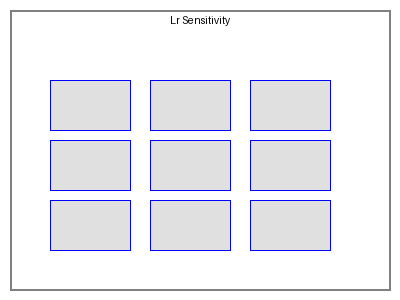
\includegraphics[width=0.45\textwidth]{assets/figures/lr_sensitivity.png}
    }
    \subfloat[批次大小]{
        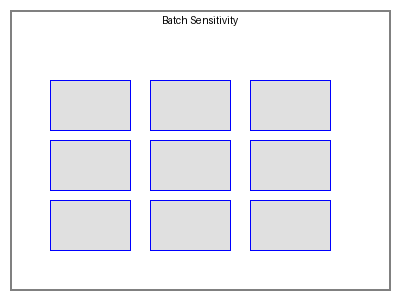
\includegraphics[width=0.45\textwidth]{assets/figures/batch_sensitivity.png}
    }
    \caption{超参数敏感性分析}
    \label{fig:hyperparam}
\end{figure}

\chapter{代码实现补充说明}

\section{模型定义核心代码}

以下是改进轻量化模块的核心实现代码：

\begin{verbatim}
// Enhanced Lite Block 核心实现
class EnhancedLiteBlock(nn.Module):
    def __init__(self, in_channels, out_channels, stride=1):
        super().__init__()
        # 深度可分离卷积
        self.dw_conv = nn.Conv2d(in_channels, in_channels, 3, 
                                 stride=stride, padding=1, 
                                 groups=in_channels)
        # 通道注意力
        self.ca = ChannelAttention(in_channels)
        # 逐点卷积
        self.pw_conv = nn.Conv2d(in_channels, out_channels, 1)
        # 增强残差连接
        if stride != 1 or in_channels != out_channels:
            self.shortcut = nn.Conv2d(in_channels, out_channels, 1, stride)
        else:
            self.shortcut = nn.Identity()
    
    def forward(self, x):
        identity = self.shortcut(x)
        out = self.dw_conv(x)
        out = self.ca(out)
        out = self.pw_conv(out)
        return out + identity
\end{verbatim}

\section{实验环境详细配置}

\begin{itemize}
    \item \textbf{操作系统}：Ubuntu 20.04 LTS
    \item \textbf{CPU}：Intel Xeon Gold 6248R @ 3.00GHz
    \item \textbf{GPU}：NVIDIA Tesla V100 32GB
    \item \textbf{深度学习框架}：PyTorch 2.0.1
    \item \textbf{Python版本}：3.10.12
    \item \textbf{CUDA版本}：11.8
\end{itemize}
